\documentclass[polish,envcountsect,10pt]{article}

   	\usepackage[T1]{fontenc}
   	\usepackage{polski}
    \usepackage{babel}
	\usepackage{subfigure}
	\usepackage{graphicx}
	\usepackage{geometry}
	\usepackage{wrapfig}
	
\title{Wizualizator topologii - instrukcja dla nauczyciela}

\author{inż. Aleksandra Wójcikowska \and inż. Michał Łubiński \and inż. Michał Czarnecki \and inż. Wojciech Baranowski}

\date{\today}
\begin{document}

\maketitle

\tableofcontents

\section{Przygotowanie sprzętu}

Przed przystąpieniem do konfigurowania środowiska laboratoryjnego należy przygotować sprzęt przeznaczony zarówno do użytku przez studentów, jak i prowadzących w celu sprawnej konfiguracji. Wymagane jest posiadanie następujących komponentów:
\begin{itemize}
	\item $3N + 1$ komputerów stacjonarnych wyposażonych w kartę sieciową oraz napęd DVD,
	\item $2N$ przełączników marki cisco (preferowanie Cisco Catalyst 3560),
	\item $N$ przełączników marki innej, niż cisco (preferowanie Planet),
	\item $N + 1$ przełączników służących jako szkielet sieci konfiguracyjnej (preferowanie Cisco Catalyst 3560),
\end{itemize}
gdzie $N$ jest liczbą stanowisk, przy których będą pracowali studenci (jedno stanowisko przeznaczone jest dla trzech studentów).

\subsection{Konfiguracja komputerów}

W pierwszej kolejności należy uruchomić system operacyjny w wersji live. Przykładem takiego systemu jest Kali Linux 2024.1. Następnym krokiem jest instalacja narzędzi wymaganych do przeprowadzenia laboratorium:
\begin{verbatim}
	sudo apt update
	sudo apt upgrade
	sudo apt install ssh
	sudo apt install net-tools 
	sudo apt install nmap
	sudo apt install lldpd
\end{verbatim}

Ostatnim krokiem jest uruchomienie klienta ssh, poprzez wykonanie komendy
\begin{verbatim}
	sudo systemctl start ssh
\end{verbatim}
pozwoli to na zdalny dostęp do urządzenia w przypadku, gdy konieczna okaże się konfiguracja systemu podczas trwania zajęć. 

\subsection{Konfiguracja przełączników Cisco}

Na początek warto przywrócić przełączniki do ustawień fabrycznych. W tym celu należy przytrzymać przycisk $mode$ przez 10-15 sekund. Następnie przełącznik nalezy podłączyć do dowolnego komputera używając portu szeregowego. Po podłączeniu na komputerze należy zainstalować narzędzie umożliwiające komunikację powiędzy urządzeniami:
\begin{verbatim}
	sudo apt install screen
\end{verbatim}
a następnie je uruchomić:
\begin{verbatim}
	sudo screen \dev\ttyUSB0
\end{verbatim}
W tym momencie na ekranie powinien wyświetlić się znak zachęty przełącznika. Następnym krokiem jest skonfigurowanie usługi ssh. Poniższe kroki przedstawiają przykładową konfigurację:
\begin{verbatim}
	enable
	conf t
	hostname NAZWA_HOSTA
	ip domain-name NAZWA_DOMENOWA
	crypto key generate rsa // Po wykonaniu komendy należy podać długość klucza.
	                        // Koniecznie musi być ona niemniejsza, niż 1024,
	                        // gdyż w przeciwnym wypadku klucz nie będzie mógł
	                        // zostać użyty przez ssh w wersji 2
	line vty 0 4
	transport input ssh
	login local
	password HASŁO
	line console 0
	logging synchronous
	login local
	username NAZWA_UŻYTKOWNIKA password HASŁO
	enable secret HASŁO
	ip ssh version 2
	write memory
\end{verbatim}
frazy zapisane wielkimi literami należy uzupełnić we własnym zakresie. W dalszej części instrukcji przyjęto, że wypełniono je frazą $cisco$.

\subsection{Konfiguracja przełączników Planet}

W przypadku wyboru przełączników planet, zresetowanie urządenia polega na przytrzymaniu przycisku $reset$ do momentu, aż zapali się 10 kontrolek z lewej strony. Na przełączniku najłatwiej jest dokonać konfiguracji za pomocą interfejsu sieciowego. W tym celu urządzenie należy podłączyć do komputera przy użyciu dowolnego z portów, a następnie wykorzystać panel konfiguracyjny dostępny pod jego adresem (domyślnie $192.168.0.100$). Aby urządzenia mogły się komunikować konieczne koże być nadanie komputerowi adresu z podsieci $192.168.0.0/24$. W tym celu należy zastosować komendę:
\begin{verbatim}
	sudo ip addr add 192.168.0.X/24 dev NAZWA_INTERFEJSU
\end{verbatim}
gdzie X jest dowolną liczbą z zakresu od 1 do 254 z pominięciem 100. Wchodząc przeglądarką pod adres 192.168.0.100 powinien wyświetlić się panel logowania do interfejsu przełącznika. Domyślnym loginem oraz hasłem jest $admin$. W panelu należy wyszukać zakładkę $security$, a następnie $ssh$. Ostatnim krokiem jest zmiana wartosci pola $mode$ z $disabled$ na $enabled$ oraz zapisanie konfiguracji przyciskiem $save$.

\subsection{Konfiguracja komputera zarządzającego}

W przypadku komputera służącego do zarządzania siecią należy poczynić dodatkowe kroki konfiguracyjne. Komputer ten powinien posiadać dodatkowy interfejs sieciowy umożliwiający połączenie urządzenia z internetem. Dobrą praktyką może okazać się zrezygnowanie z systemu operacyjnego w wersji $live$ na poczet przeprowadzenia pełnej instalacji systemu. Dzięki temu w razie awarii konfiguracja nie zostanie utracona.

\subsubsection{Instalacja oprogramowania}

Pierwszym krokiem jest instalacja wszystkich potrzebnych narzędzi. Przeprowadzić ją można z wykorzystaniem następujących komend:
\begin{verbatim}
	sudo apt update
	sudo apt upgrade
	sudo apt install net-tools 
	sudo apt install nmap
	sudo apt install isc-dhcp-server radvd
	sudo apt install vim
	sudo apt install curl
	sudo apt install iptables
\end{verbatim}

\subsubsection{DHCP}

Następnym krokiem jest konfiguracja serwera DHCP, a co za tym idzie adresacja urządzeń w sieci. Warto nadmienić, że za pośrednictwem adresów MAC, urządzeniom zostaną przypisane stałe adresy IP. Zastosowanie serwera DHCP w tym przypadku sprowadzać się będzie głównie do przywracania adresów urządzeń w przypadku awarii części infrastruktury bądź restartu urządzeń. Jako przestrzeń sieciowa wykorzystana zostanie podsieć $10.0.0.0/24$. Poniżej przedstawiono sposób adresacji:
\begin{itemize}
	\item $10.0.0.1$ - komputer zarządzający, tożsamy z bramą,
	\item $10.0.0.2$ - główny przełącznik zarządzający,
	\item $10.0.0.G0$ - przełącznik zarządzający w grupie o numerze $G$,
	\item $10.0.0.G1$, $10.0.0.G2$, $10.0.0.G3$ - komputery w grupie $G$,
	\item $10.0.0.G4$, $10.0.0.G5$ - przełączniki Cisco w grupie $G$,
	\item $10.0.0.G6$ - przełącznik Planet w grupie $G$.
\end{itemize}
W dalszej kolejności należy utworzyć plik konfiguracyjny $/etc/dhcp/dhcpd.conf$ z następującą zawartością:
\begin{verbatim}
	option domain-name "lab.local"
	default-lease-time 60;
	max-lease-time 900;
	authoritative;
	subnet 10.0.0.0 netmask 255.255.255.0 {
	  range 10.0.0.100 10.0.0.200;
	  option routers 10.0.0.1;
	}

	// poniższy fragment należy powielić dla kazdego urządzenia

	host NAZWA_URZĄDZENIA {
	  hardware ethernet ADRES_MAC_URZĄDZENIA;
	  fixed-address DOCELOWY_ADRES_URZĄDZENIA;
	}
\end{verbatim}
Serwer uruchamia się wydając polecenie
\begin{verbatim}
	sudo systemctl start isc-dhcp-server
\end{verbatim}
Aby przydzielić komputerowi zarządzającemu odpowiednie IP, wydaje się polecenie
\begin{verbatim}
	sudo dhclient -v NAZWA_INTERFEJSU
\end{verbatim}

\subsubsection{Routing}

W celu zapewnienia wszystkim urządzeniom dostępu do internetu należy skonfigurować routing pomiędzy interfejsami komputera zarządzającego. Na potrzeby instrukcji interfejs komputera, przez który łączy się on z internetem oznaczono jako $ZEWNĘTRZNY$, natomiast interfejs, poprzez który jest on połączony z siecią wewnętrzną jako $WEWNĘTRZNY$. Konfigurację wykonuje się za pomocą następujących poleceń:
\begin{verbatim}
	sudo ip route add 10.0.0.0/24 via 10.0.0.1 dev WEWNĘTRZNY
	sudo ip route add default via ZEWNĘTRZNY
	sudo iptables -t nat -A POSTROUTING -s '10.0.0.0/24' -o ZEWNĘTRZNY -j MASQUERADE
	sudo iptables -A FORWARD -i WEWNĘTRZNY -o ZEWNĘTRZNY -j ACCEPT
	sudo iptables -A FORWARD -i ZEWNĘTRZNY -o WEWNĘTRZNY -m conntrack\
	     --cstate ESTABLISHED,RELATED -j ACCEPT
\end{verbatim}
Ponadto w celu zezwolenia na przekazywanie pakietów należy wykonać następującą komendę:
\begin{verbatim}
	sudo echo 1 > /proc/sys/net/ipv4/ip_forward
\end{verbatim}

\subsection{Realizacja sieci}

Urządzenia należy połączyć w sieć wzorując się na poniższym schemacie:

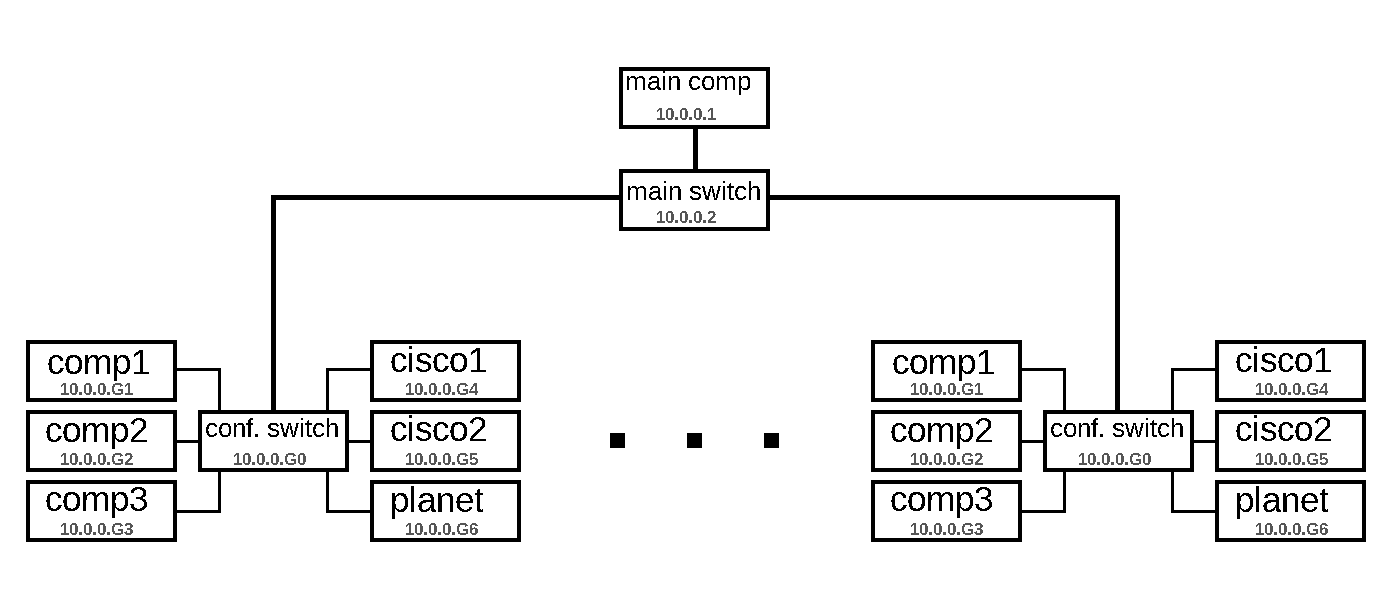
\includegraphics[width=\linewidth]{siec.png}

W celu urozmaicenia ćwiczenia zaleca się stosowanie portów o różnych numerach oraz opcjonalne rozszerzenie sieci o połączenia między przełącznikami w obszarze pojedynczej grupy.

\end{document}
